% This is Lecture Notes for PET504E Advanced Well Test Analysis
%
\documentclass{llncs}

\usepackage{graphicx}
\usepackage{framed,color}
\definecolor{shadecolor}{rgb}{0.3921,0.58431,0.9294}
\usepackage{llncsdoc}
\usepackage{savesym}
\usepackage{float}
\savesymbol{note}
\usepackage{color} % Allow text colors
\usepackage{enumerate}
\usepackage{amsmath}

%\usepackage{fullpage}
%\usepackage[finalnew]{trackchanges}
%\usepackage[finalold]{trackchanges}
%\usepackage[footnotes]{trackchanges}
%\usepackage[inline]{trackchanges}
\usepackage[margins]{trackchanges}
%\usepackage[margins, movemargins]{trackchanges}
%\usepackage[margins, adjustmargins]{trackchanges}
%
\addeditor{Murat \c{C}{\i}nar}
\restoresymbol{Trck}{note}
 \numberwithin{equation}{section}
 \numberwithin{figure}{section}
 \numberwithin{table}{section}
%
%\usepackage{nomencl}
%\makenomenclature
%
\begin{document}
    \markboth{PET504E Advanced Well Test Analysis}{PET504E Advanced Well Test Analysis}
    \thispagestyle{empty}
    \begin{flushleft}
        \LARGE\bfseries Lecture Notes\\[1cm]
    \end{flushleft}
    \rule{\textwidth}{1pt}
    \vspace{2pt}
    \begin{flushright}
        \Huge
            \begin{tabular}{@{}l}
                PET504E \\
                Advanced Well Test \\
                Analysis\\[6pt]
                {\Large January 2012}
            \end{tabular}
        \end{flushright}
    \rule{\textwidth}{1pt}

    \begin{flushleft}
        \LARGE\bfseries by\\ Prof. Dr. Mustafa Onur \\[0.5cm]
        Dr. Murat \c{C}{\i}nar\\

    \end{flushleft}
    \vfill

    \section{Introduction}
%
    The term "Well Testing" \add[Murat \c{C}{\i}nar]{as it} is used in Petroleum Industry means the measuring of a formation's
    (or reservoir's) pressure (and/or rate) response to flow from a well. The term "Well Testing"
    is generally used with the term "Pressure Transient Analysis", interchangeably. It is an indirect
    measurement technique as opposed to direct methods such as fluid sampling or coring. Well testing
    provides dynamic information on the reservoir whereas direct measurements only provide static
    information, which is not sufficient for predicting the behavior of the reservoir.\\

    Simply, the objective of well testing is to deduce quantitative information about the well/reservoir system
    under consideration from its response to a given input. Input (or input signal) is used for perturbing one or more
    wells so that the output (signal) exhibiting the response of the reservoir is obtained at the perturbated well and/or
    adjacent wells. In practice, the input is equivalent to controlling the well behavior \remove[Murat \c{C}{\i}nar]{and} created by changing
    the flow rate or the pressure at the well (Mathematically specifying the well behavior is equivalent to specifying
    a boundary condition). A common example for creating an input signal is \add[Murat \c{C}{\i}nar]{a} build up test
    \change[Murat \c{C}{\i}nar]{in which}{where} we change the rate to zero by shutting-in the well. Reservoir response,
    \remove[Murat \c{C}{\i}nar]{which is} also called output signal, to a given input is monitored by measuring the
    pressure change (or rate change) at the \remove[Murat \c{C}{\i}nar]{same}  well. This process is illustrated as,

    \begin{figure}[h]
        \setlength{\unitlength}{0.14in} % selecting unit length
        \centering % used for centering Figure
        \begin{picture}(32,15) % picture environment with the size (dimensions)
        % 32 length units wide, and 15 units high.
            \put(3,4){\framebox(6,3){Input}}
            \put(13,4){\framebox(6,3){System}}
            \put(23,4){\framebox(6,3){Output}}
            \put(14,3){(Unknown)}
            \put(6,1){I}
            \put(16,1){S}
            \put(26,1){O}
            \put(9,5.5){\vector(1,0){4}}
            \put(19,5.5){\vector(1,0){4}}
            \put(9,1){\vector(1,0){4}}
            \put(19,1){\vector(1,0){4}}
        \end{picture}
        \caption{Block diagram ?????}
        \label{input_output} % label to refer figure in text
    \end{figure}

    Typical examples for input and output signals as used in petroleum industry are shown in Fig. \ref{Transient_phenomena}.
    \begin{figure}
        \begin{center}
        \includegraphics[scale=0.75]{Transient_phenomena.pdf}
        \caption{Typical input and output signals - Transient phenomena.}
        \label{Transient_phenomena}
        \end{center}
    \end{figure}


    From reservoir response as monitored by the "output signal", we would like to determine information related to the followings:
    \begin{itemize}
        \item Fluid in place; pore volume, ${\phi}hA$.
        \item Ability of reservoir to transfer fluid, $kh$ (or transmissibility, $\frac{kh}{\mu}$).
        \item Determination of average reservoir \change[Murat \c{C}{\i}nar]{average}{pressure}, $\overline{P}$, which is the driving force in the reservoir \Trcknote[Murat \c{C}{\i}nar]{Based upon the explanation you gave about the pressure decline recently, I am not sure if this statement is correct.}
        \item Prediction of rate versus time data.
        \item Initial recovery, is the reservoir worth producing.
        \item Is there any damage around the wellbore impeding the flow? skin factor, $s$.
        \item Reservoir description (type of reservoir, flow boundaries (faults)).
        \item Distance to fluid interface \change[Murat \c{C}{\i}nar]{which}{that} is important determining swept zone for secondary and tertiary methods.
    \end{itemize}
    Interpretation of well test data consist of basically three steps:

    \begin{enumerate}[(i)]
        \item Determination of the one most appropriate reservoir / wellbore (mathematical) model \change[Murat \c{C}{\i}nar]{to}{of} the actual system. We also call such a model as the interpretation model. \change[Murat \c{C}{\i}nar]{Here our hope is that the model chosen will produce an output signal to a given input which is as close as possible to that of the actual system.}{Here our intention is to find a representative mathematical model that reproduces, as close as possible, the output of the actual system for a given input.} This is known as the inverse problem. \add[Murat \c{C}{\i}nar]{We are trying to obtain information about the physical system by using observed measurements.} Unfortunately, the solution of inverse problem often yields non-unique results. \change[Murat \c{C}{\i}nar]{With}{By} non-unique results, we mean that several different interpretation models \change[Murat \c{C}{\i}nar]{can}{may} generate an output signal (response) to a given input \change[Murat \c{C}{\i}nar]{which}{that} is similar (or identical) to that of the actual system. The inverse problem can be represented by the following equation.

        \begin{equation}
            \Sigma ={O}/{I}\;\approx S
            \label{InvP}
        \end{equation}

            where $\Sigma$ denotes the interpretation model, $S$ denotes the actual system. In inverse problem, as can be seen from Eq.\ref{InvP}, it may be possible to obtain the same outputs to a given $I$ for different $\Sigma_{i}$'s\change[Murat \c{C}{\i}nar]{. However}{,however}, the number of alternative models (solutions) can be reduced as the number and the range of output signal measurements.\\

        \item Once the appropriate model is determined, estimate the parameters of the actual system $S$. \change[Murat \c{C}{\i}nar]{Such parameters can be}{These parameters are} $kh$, $s$, $\phi$, $C$, $\lambda$, $w$ etc. This is known as \remove[Murat \c{C}{\i}nar]{the}parameter estimation\remove[Murat \c{C}{\i}nar]{problem}\change[Murat \c{C}{\i}nar]{.  It is}{ and} achieved by adjusting the parameters of the model by different \add[Murat \c{C}{\i}nar]{mathematical} methods to obtain an output signal, $\Omega$, that is always qualitatively identical (within some tolerance) to that of \add[Murat \c{C}{\i}nar]{the} actual system, $O$. The computation of $\Omega$ is known as
            the "\change[Murat \c{C}{\i}nar]{direct}{forward} problem" in mathematics. Contrary to the inverse problem, the solution of the \change[Murat \c{C}{\i}nar]{direct}{forward} problem is always unique for a given system; that is,
        \begin{equation}
            I\times \Sigma =\Omega \approx 0
            \label{ForP}
        \end{equation}
            The adjusted parameters of the interpretation model are assumed to represent the parameters of the real system $S$.  \Trcknote[Murat \c{C}{\i}nar]{I think we should discuss this phrase. Does the real system have any parameters? I do not think so... This is something conceptual we need to think about}
        \item Validate the results of the interpretation. This can be achieved by using the parameters determined from part $(ii)$ in the model
              to generate output signals for the entire range of \add[Murat \c{C}{\i}nar]{the} test and by comparing these outputs with the \change[Murat \c{C}{\i}nar]{measured ones}{physical measurements}.
    \end{enumerate}

    \begin{figure}
        \begin{center}
        \includegraphics[scale=1]{Build_up.pdf}
        \caption{Parameters estimated based on the analysis of buildup data.}
        \label{Build_up}
        \end{center}
    \end{figure}

    \change[Murat \c{C}{\i}nar]{To illustrate an example of direct and inverse problems, let's consider single phase flow in a closed cylindrical reservoir produced by a single well at the center.}{Now we consider single phase flow in a cylindrical reservoir produced by a well at the center.} The\change[Murat \c{C}{\i}nar]{pd.E}{partial differential equation (p.d.e.)} describing the flow is given by,
    \begin{equation}
        \frac{1}{r}\frac{\partial }{\partial r}\left( \frac{kr}{\mu }\frac{\partial p}{\partial r} \right)=\phi {{c}_{t}}\frac{\partial p}{\partial t}
        \label{A}
    \end{equation}
    or if $k$, $\mu$ are constant,
    \begin{equation}
        \frac{1}{r}\frac{\partial }{\partial r}\left( r\frac{\partial p}{\partial r} \right)=\frac{\phi {{c}_{t}}\mu }{k}\frac{\partial p}{\partial t}=\frac{1}{\eta }\frac{\partial p}{\partial t}
        \label{B}
    \end{equation}

    \change[Murat \c{C}{\i}nar]{$\eta =\frac{\phi {{c}_{t}}\mu }{k}$}{$\eta =\frac{k}{\phi {{c}_{t}}\mu }$ } is the hydraulic diffusivity\change[Murat \c{C}{\i}nar]{which is}{;} a measure of the \change[Murat \c{C}{\i}nar]{rapidity with}{speed at} which a pressure disturbance \add[Murat \c{C}{\i}nar]{propagates} through the formation.
    If we specify, $k$, $\phi$, $c_{t}$, $\mu$, and the flow rate, then $p(r,t)$ is uniquely determined. This is an example for the \change[Murat \c{C}{\i}nar]{direct}{forward} problem.\\

    Inverse problem, given $q$ and $p$, \add[Murat \c{C}{\i}nar]{helps us to}
    \begin{enumerate}
        \item determine the p.d.e. that describes the reservoir best
        \item find $k$, $\phi$, etc.
    \end{enumerate}

    \remove[Murat \c{C}{\i}nar]{
    During the past ten years, a lot of work has been done to develop models to a wide variety of reservoir / well configurations such as fractures, layered reservoirs, multiple porosities (composite zones), fractured wells, slanted and horizontal wells, etc. Well testing literature is almost complete for single phase problems, but some work needs to be done for multi-phase problems and heterogeneous reservoir systems.\\

    Recently, people are much focused on the model recognition problem and the computer-aided parameter estimation by using non-linear regression techniques. Pressure derivatives and integrals are proven to be very useful in identifying the appropriate mathematical model from flow regime analysis. Currently, a lot of work is on artificial intelligence (AI) techniques for model recognition, such as rule-based expert and neural networks approaches.}

    \Trcknote[Murat \c{C}{\i}nar]{I added the following paragraph}Analytical solutions have been presented in the literature for a variety of different well and reservoir settings for single phase flow. A summary of these responses are given by Bourdet \cite{Bourdet_2002_1}.

    \begin{figure}
        \begin{center}
        \includegraphics[scale=0.6]{Homogenous_vs_Heterogenous_dp.pdf}
        \caption{Homogeneous vs heterogeneous reservoir, pressure difference .}
        \label{Homogenous_vs_Heterogenous_dp}
        \end{center}
    \end{figure}

    \begin{figure}
        \begin{center}
        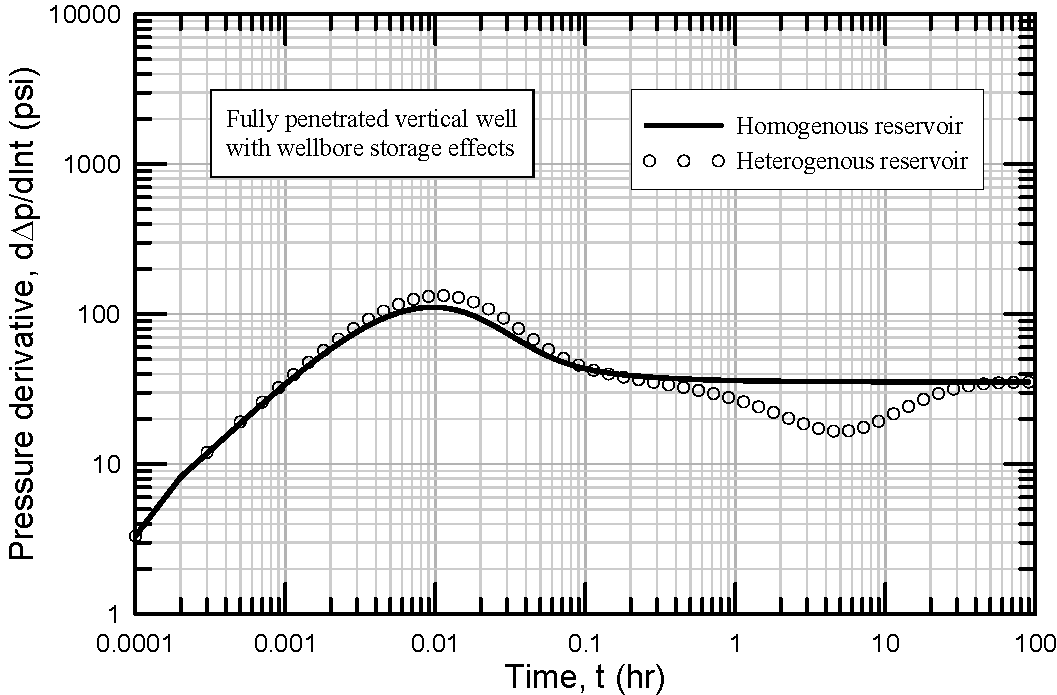
\includegraphics[scale=0.6]{Homogenous_vs_Heterogenous_dpder.pdf}
        \caption{Homogeneous vs heterogeneous reservoir - logarithmic derivative.}
        \label{Homogenous_vs_Heterogenous_dpder}
        \end{center}
    \end{figure}

    \begin{figure}
        \begin{center}
        \includegraphics[scale=0.3]{Flow_Chart1.pdf}
        \caption{Flow diagram of computer aided parameter estimation.}
        \label{Flow_Chart1}
        \end{center}
    \end{figure}

    \section{Flow Equations}

    In this chapter, we will derive the equations which describe the fluid flow in porous media. Such equations are derived from the conservation of mass and the momentum equation as given by Darcy's semi-empirical equation. With the exception of thermal recovery schemes, all well-testing models assume isothermal conditions in the reservoir and thus the energy conservation is not needed.
    \subsection{Conservation of mass}
    For a single phase fluid \remove[Murat \c{C}{\i}nar]{(or a fluid composed of one hydrocarbon component)}, the mathematical form of the mass balance in porous media is given by
    \begin{equation}
        -\nabla \cdot \left( \rho \mathbf{v} \right)=\frac{\partial \left( \rho \phi  \right)}{\partial t}
        \label{continuity}
    \end{equation}
    \Trcknote[Murat \c{C}{\i}nar]{I removed the constant -5.615 from the equation}
    where $\rho$ is the density of the fluid in \change[Murat \c{C}{\i}nar]{$lbm/ft^{3}$}{$\mathbf{M}/\mathbf{L}^{3}$} and $\mathbf{v}$ is the fluid velocity vector in \change[Murat \c{C}{\i}nar]{$RB/ft^{2}day$}{$\mathbf{L}/\mathbf{T}$}. Note that the units of Eq. \ref{continuity} is \change[Murat \c{C}{\i}nar]{$lbm/ft^{3}day$}{$\mathbf{M}/\mathbf{L}^3\mathbf{T}$} It is also important to note that Eq. \ref{continuity} applies for any coordinate system and can be derived either from a mass balance done on a control volume for a coordinate system under consideration or from \remove[Murat \c{C}{\i}nar]{a} divergence theorem (or Gauss Theorem see Supplement II).

    In\change[Murat \c{C}{\i}nar]{x-y-x}{Cartesian} coordinate system,
    \begin{equation}
        \nabla \cdot \left( \rho \mathbf{v} \right)=\frac{\partial }{\partial x}\left( \rho {{v}_{x}} \right)+\frac{\partial }{\partial y}\left( \rho {{v}_{y}} \right)+\frac{\partial }{\partial z}\left( \rho {{v}_{z}} \right)
        \label{continuity_Cartesian}
    \end{equation}

    In\change[Murat \c{C}{\i}nar]{r-$\theta$-z}{cylindrical} coordinate system,
    \begin{equation}
        \nabla \cdot \left( \rho \mathbf{v} \right)=\frac{1}{r}\frac{\partial }{\partial r}\left( r\rho {{v}_{r}} \right)+\frac{1}{r}\frac{\partial }{\partial \theta }\left( \rho {{v}_{\theta }} \right)+\frac{\partial }{\partial z}\left( \rho {{v}_{z}} \right)
        \label{continuity_cylindrical}
    \end{equation}
    \Trcknote[Murat \c{C}{\i}nar]{typo in the equation corrected}
    \subsection{Conservation of momentum in porous media}
    The principle of momentum conservation is described by the equation of motion. For most hydrocarbon fluids, the shear stress - shear rate behavior \change[Murat \c{C}{\i}nar]{can be}{is} described by the Newton's law of friction, combined with the equation of motion, results in the well known Navier-Stokes equation. Solution of the Navier-Stokes equation with the appropriate boundary conditions yields the velocity distribution of a given problem. Although, it is possible to solve Navier-Stokes in pipe flow, it is almost impossible to solve due to complexity of the pore geometry and its distribution. This hinders the formation of the boundary conditions for flow through a porous medium. Therefore, a different approach \change[Murat \c{C}{\i}nar]{must be}{is} taken. In 1856, \change[Murat \c{C}{\i}nar]{a French hydraulic engineer Henry} Darcy discovered that \change[Murat \c{C}{\i}nar]{the velocity vector and the pressure gradient for a single phase viscous flow}{for a single phase viscous flow in porous media, the velocity is proportional to the pressure gradient with a proportionality constant $k$. The general form of Darcy's Law including gravity effects is given by Eq.}\ref{Darcy's_Law}.
    \begin{equation}
        \mathbf{v}=-\frac{\mathbf{k}}{\mu }\left( \nabla p-\rho g\nabla z' \right)
        \label{Darcy's_Law}
    \end{equation}
    \Trcknote[Murat \c{C}{\i}nar]{I removed the filed unit constants}
    where $\mathbf{v}$ is defined as a volumetric flow rate across a unit cross-section area (solid+fluid) averaged over a small region of space. The unit of $\mathbf{v}$ is in \change[Murat \c{C}{\i}nar]{$RB/ft^{2}day$}{$\mathbf{L}/\mathbf{T}$}. Eq. \ref{Darcy's_Law} yield\add[Murat \c{C}{\i}nar]{s} a velocity vector \change[Murat \c{C}{\i}nar]{which}{that} replaces the solution of Navier-Stokes equation. In Eq. \ref{Darcy's_Law} $\mathbf{k}$ is \change[Murat \c{C}{\i}nar]{a}{the} permeability tensor. Operationally, $\mathbf{k}$ acts like a matrix in \change[Murat \c{C}{\i}nar]{x-y-z}{coordinate system}, we usually \change[Murat \c{C}{\i}nar]{use}{assume}
    \begin{equation*}
        \mathbf{k}\,\nabla p=\begin{bmatrix}
             {{k}_{x}} & 0 & 0  \\
             0 & {{k}_{y}} & 0  \\
             0 & 0 & {{k}_{z}}  \\
            \end{bmatrix}\begin{bmatrix}
            & \frac{\partial p}{\partial x} \\
            & \frac{\partial p}{\partial y} \\
            & \frac{\partial p}{\partial z} \\
            \end{bmatrix} = \begin{bmatrix}
            & {{k}_{x}}\frac{\partial p}{\partial x} \\
            & {{k}_{y}}\frac{\partial p}{\partial y} \\
            & {{k}_{z}}\frac{\partial p}{\partial z} \\
            \end{bmatrix}
        \label{Permeability_Tensor}
    \end{equation*}
    \begin{equation*}
        \nabla {z}'=\begin{bmatrix}
        & \frac{\partial {z}'}{\partial x} & \\
        & \frac{\partial {z}'}{\partial y} & \\
        &\frac{\partial {z}'}{\partial z}  &
        \end{bmatrix}
        \label{Z}
    \end{equation*}
    where, ${z}'$ is the direction in which gravity acts, i.e., the direction towards the center of the earth.
    In \change[Murat \c{C}{\i}nar]{x-y-z}{Cartesian} coordinate system, \remove[Murat \c{C}{\i}nar]{Eq. 2.5} for each velocity component,
    \begin{equation}
    {{v}_{\xi }}=-\frac{{{k}_{\xi }}}{\mu }\left( \frac{\partial p}{\partial \xi }-\rho g\frac{\partial z'}{\partial \xi } \right),\quad \xi =x,y,z
        \label{Darcy_velocity}
    \end{equation}

    We generally denote $\gamma$ as the specific weight of fluid and define as,
    \begin{equation*}
        \gamma =\rho g
        \label{Specific_weight}
    \end{equation*}

    It follows from Eq. \ref{Darcy_velocity}, \ref{continuity_Cartesian}, and \ref{continuity} that the p.d.e. describing conservation of mass in \remove[Murat \c{C}{\i}nar]{x-y-z}{Cartesian} coordinate system is
    \begin{equation}
        \begin{split}
            & \,\,\,\,\,\,\ \frac{\partial }{\partial x}\left[ \rho \frac{{{k}_{x}}}{\mu }\left( \frac{\partial p}{\partial x}-\gamma \frac{\partial z'}{\partial x} \right) \right] \\
            & +\frac{\partial }{\partial y}\left[ \rho \frac{{{k}_{y}}}{\mu }\left( \frac{\partial p}{\partial y}-\gamma \frac{\partial z'}{\partial y} \right) \right] \\
            & +\frac{\partial }{\partial z}\left[ \rho \frac{{{k}_{z}}}{\mu }\left( \frac{\partial p}{\partial z}-\gamma \frac{\partial z'}{\partial z} \right) \right]=\frac{\partial }{\partial t}\left( \rho \phi  \right) \\
        \end{split}
    \label{Continuity_Darcy}
    \end{equation}

    In \change[Murat \c{C}{\i}nar]{r-z}{Cylindrical} coordinates (neglecting flow in $\theta$ direction)
    \begin{equation}
        \,\,\,\,\,\frac{1}{r}\,\frac{\partial }{\partial r}\left[ r\frac{{{k}_{r}}}{\mu }\rho \left( \frac{\partial p}{\partial r}-\gamma \frac{\partial z'}{\partial r} \right) \right]+\frac{\partial }{\partial z}\left[ \frac{{{k}_{z}}}{\mu }\rho \left( \frac{\partial p}{\partial z}-\gamma \frac{\partial z'}{\partial z} \right) \right]=\frac{\partial }{\partial t}\left( \rho \phi  \right)
    \label{Continuity_Darcy_Cylindrical}
    \end{equation}

    \vspace{15pt}
    \large{\textbf{Remark on gravity term:}}\\
    \rule{\textwidth}{1pt}
    \begin{figure}
        \begin{center}
            \includegraphics[scale=1]{Z_Aside.pdf}
        \label{Z_Aside}
        \end{center}
    \end{figure}
    In \change[Murat \c{C}{\i}nar]{r-$\theta$-z}{Cylindrical} coordinates,\change[Murat \c{C}{\i}nar]{if reservoir is horizontal; i.e. $\theta'=0$}{assume $z$ and $z'$ are in the same direction then,}
    \begin{equation*}
        \frac{\partial z'}{\partial r}=\frac{\partial z'}{\partial \theta }=0\quad and\quad \frac{\partial z'}{\partial z}=1
    \end{equation*}
    \change[Murat \c{C}{\i}nar]{If we had a dip angle $\theta'$}{if the reservoir is dipping with an angle of $\theta'$},
    \begin{equation*}
        \frac{\partial z'}{\partial r}=\sin \theta '\quad \frac{\partial z'}{\partial \theta }=\cos \theta '\quad \frac{\partial z'}{\partial z}=\cos \theta '
    \end{equation*}\\
    \rule{\textwidth}{1pt}\\
    \vspace{15pt}

    \change[Murat \c{C}{\i}nar]{If we}{Now} consider a single well \change[Murat \c{C}{\i}nar]{in}{at} the center of a cylindrical reservoir, then Eq. \ref{Continuity_Darcy_Cylindrical} correctly describes the fluid flow for both partially penetrating and fully penetrating cases, see Fig \ref{PartialvsFullPenet}.\\
    \begin{figure}
        \begin{center}
        \includegraphics[scale=0.6]{PartialvsFullPenet.pdf}
        \caption{(a) Fully penetrated vertical well. (b) Partially penetrated vertical well.}
        \label{PartialvsFullPenet}
        \end{center}
    \end{figure}
    \remove[Murat \c{C}{\i}nar]{Recalling our general continuity equation for the single phase flow gives,}
    \add[Murat \c{C}{\i}nar]{Now define formation volume factor $B$ as,}

    \begin{equation}
        B=\frac{{{V}_{reservoir}}}{{{V}_{SC}}}=\frac{{m}/{\rho }\;}{{{{m}/{\rho }\;}_{SC}}}=\frac{{{\rho }_{SC}}}{\rho }\quad ;\quad {{\rho }_{SC}}\,\text{is}\,\text{constant}
    \label{Formation_Volume_Factor}
    \end{equation}

    \remove[Murat \c{C}{\i}nar]{which we call it as Formation volume factor, then we can write Equation (2.8) as}
    \add[Murat \c{C}{\i}nar]{Recall general continuity equation,} Eq. \ref{continuity} and insert Eq. \ref{Formation_Volume_Factor}, then we have,

    \begin{equation}
        -\nabla \cdot \left( \frac{\mathbf{v}}{B} \right)=\frac{\partial }{\partial t}\left( \frac{\phi }{B} \right)
    \label{Continuity_B}
    \end{equation}

    $B=B(p)$, $\rho=\rho(p)$, and $\phi=\phi(p)\rightarrow$ single valued functions of $p$
    \add[Murat \c{C}{\i}nar]{Expanding right hand side (RHS) of} Eq. \ref{Continuity_B},

    \begin{equation}
        \begin{split}
            \frac{\partial }{\partial t}\left( \frac{\phi }{B} \right)&= \phi \frac{\partial }{\partial t}\left( \frac{1}{B} \right)+\frac{1}{B}\frac{\partial \phi }{\partial t} \\
            &=\phi \left( -\frac{1}{{{B}^{2}}}\frac{dB}{dp} \right)\frac{\partial p}{\partial t}+\frac{1}{B}\frac{d\phi }{dt}\frac{\partial p}{\partial t} \\
            &=\frac{\phi }{B}\left( -\frac{1}{B}\frac{dB}{dp}+\frac{1}{\phi}\frac{d\phi }{dt} \right)\frac{\partial p}{\partial t} \\
    \end{split}
    \label{Continuity_B_Expand_RHS}
    \end{equation}
    \Trcknote[Murat \c{C}{\i}nar]{Typo in Eq corrected.}
    \remove[Murat \c{C}{\i}nar]{but} Fluid and rock compressibilities are defined, respectively, by,

    \begin{equation}
    {{c}_{fluid}}=-\frac{1}{V}\frac{dV}{dp}=-\frac{1}{B}\frac{dB}{d\rho }=\frac{1}{\rho }\frac{d\rho }{dp}
    \label{Fluid_compressibility}
    \end{equation}

    \begin{equation}
    {{c}_{r}}={{c}_{f}}=\frac{1}{\phi }\frac{d\phi }{dp}
    \label{Rock_compressibility}
    \end{equation}

    (here $p$ is the fluid pressure in the pore, therefore, $\frac{d\phi }{dp}>0$.) \\
    Using Eqs. \ref{Fluid_compressibility} and \ref{Rock_compressibility} in Eq. \ref{Continuity_B_Expand_RHS} and the resulting equation in Eq. \ref{Continuity_B} gives,

    \begin{equation}
        -\nabla \cdot \left( \frac{\mathbf{v}}{B} \right)=\frac{\phi {{c}_{t}}}{B}\frac{\partial p}{\partial t}
    \label{Continuity_B_ct}
    \end{equation}

    \add[Murat \c{C}{\i}nar]{Note that here the total compressibility $c_{t}$ is defined as ${{ c }_{t}}={{c}_{fluid}}+{{c}_{r}}$. Under the assumptions of Darcy's Law we have,}

    \begin{equation}
        \nabla \cdot \left( \frac{\mathbf{k}}{\mu B}\left( \nabla p-\gamma\nabla z' \right) \right)=\frac{\phi {{c}_{t}}}{B}\frac{\partial p}{\partial t}
    \label{Continuity_B_ct_Darcy}
    \end{equation}
    
    Now assuming negligible gravity effects and $k/\mu$ is constant then,
    
    \begin{equation}
        \frac{k}{\mu }\nabla \cdot \left( \rho \nabla p \right)=\phi {{c}_{t}}\rho \frac{\partial p}{\partial t}
    \label{Continuity_B_ct_Darcy_No_Gravity1}
    \end{equation}    
    
    \change[Murat \c{C}{\i}nar]{If we assume}{Assuming} $c{{\left( \nabla p \right)}^{2}}$ is small here $c=\frac{1}{\rho }\frac{\partial \rho }{\partial p}$, Eq. \ref{Continuity_B_ct_Darcy_No_Gravity1} is well approximated by
    
    \begin{equation}
        \frac{k}{\mu }{{\nabla }^{2}}p=\phi {{c}_{t}}\frac{\partial p}{\partial t}
    \label{Continuity_B_ct_Darcy_No_Gravity1_approx}
    \end{equation}     
    
    \vspace{15pt}
    \large{\textbf{Remark on coordinate systems:}}\\
    \rule{\textwidth}{1pt}
    
    \begin{equation*}
        {{\nabla }^{2}}p=\frac{{{\partial }^{2}}p}{\partial {{x}^{2}}}+\frac{{{\partial }^{2}}p}{\partial {{y}^{2}}}+\frac{{{\partial }^{2}}p}{\partial {{z}^{2}}}\quad \text{in Cartesian coordinates}
    \label{Laplacian_Cartesian}
    \end{equation*}     

    \begin{equation*}
        {{\nabla }^{2}}p=\frac{1}{r}\frac{\partial }{\partial r}\left( r\frac{\partial p}{\partial r} \right)+\frac{1}{{{r}^{2}}}\frac{{{\partial }^{2}}p}{\partial {{\theta }^{2}}}+\frac{{{\partial }^{2}}p}{\partial {{z}^{2}}}\quad \text{in cylindrical coordinates}
    \label{Laplacian_Cylindrical}
    \end{equation*} 

    \begin{equation*}
        \begin{split}
    & {{\nabla }^{2}}p=\frac{1}{{{r}^{2}}}\frac{\partial }{\partial r}\left( {{r}^{2}}\frac{\partial p}{\partial r} \right)+\frac{1}{{{r}^{2}}sin\theta }\frac{\partial }{\partial \theta }\left( sin\theta \frac{\partial p}{\partial \theta } \right) \\
    & +\frac{1}{{{r}^{2}}si{{n}^{2}}\theta }\frac{{{\partial }^{2}}p}{\partial {{\phi }^{2}}} \\
    \end{split}\quad \text{in spherical coordinates}
    \label{Laplacian_Spherical}
    \end{equation*}     
    
    \begin{figure}[H]
        \begin{center}
            \includegraphics[scale=0.65]{Coordinates.pdf}
        \caption{(a) Cartesian coordinates. (b) Cylindrical coordinates. (c) Spherical coordinates.}
        \label{Coordinates}
        \end{center}
    \end{figure}       
    \rule{\textwidth}{1pt}
    \vspace{15pt}    
    
    Further \change[Murat \c{C}{\i}nar]{if we assume}{assuming},
    \begin{equation}
        c=\frac{1}{\rho }\frac{\partial \rho }{\partial p}=\text{constant}
    \label{c_constant}
    \end{equation} 
    
    \begin{equation*}
        \int_{{{p}_{i}}}^{p}{cdp}=\int_{{{\rho }_{i}}}^{\rho }{\frac{1}{\rho }d\rho }
    \end{equation*}   

    \begin{equation*}
        c\left( p-{{p}_{i}} \right)=\ln \left( \frac{\rho }{{{\rho }_{i}}} \right)\quad ; \quad p_{i}\,\text{initial pressure}
    \end{equation*}    
    or
    \begin{equation}
        \rho ={{\rho }_{i}}\exp \left[ -c\left( {{p}_{i}}-p \right) \right]
    \label{rho_func}
    \end{equation}
    
    Using Taylor series representation of $\exp \left[ -c\left( {{p}_{i}}-p \right) \right]$ gives,
    \begin{equation*}    
        \begin{split}
         \rho &={{\rho }_{i}}\left[ 1-c\left( {{p}_{i}}-p \right)+\frac{{{c}^{2}}}{2}{{\left( {{p}_{i}}-p \right)}^{2}}+\cdots  \right] \\
        & ={{\rho }_{i}}\left[ 1-c\left( {{p}_{i}}-p \right)+\frac{{{c}^{2}}}{2}{{\left( {{p}_{i}}-\widetilde{p} \right)}^{2}} \right]\quad p<\widetilde{p}<{{p}_{i}} \\
        \end{split}
    \end{equation*}   
    \begin{equation}
        \rho ={{\rho }_{i}}\left[ 1-c\left( {{p}_{i}}-p \right) \right]
    \label{rho_func_2}
    \end{equation}   
    \add[Murat \c{C}{\i}nar]{Note that} $c$ is very small for oil (or liquids); $c\approx10^{-5}\sim10^{-6}$. Using Eq. \ref{rho_func_2} in Eq. \ref{Continuity_B_ct_Darcy_No_Gravity1_approx}.
    \begin{equation}
        \frac{k}{\mu }{{\nabla }^{2}}p = \phi {{c}_{t}}\frac{\partial p}{\partial t}
    \label{Continuity_B_ct_Darcy_No_Gravity1_approx_rho}
    \end{equation}     
    \subsection{Multiphase flow}
    Three distinct phases, gas, oil, and water occur i a petroleum reservoir. Varying pressure conditions (isothermal system assumed) cause a mass exchange between \remove[Murat \c{C}{\i}nar]{the}two hydrocarbon phases \add[Murat \c{C}{\i}nar]{- oil-gas} (water-oil and gas-water systems \change[Murat \c{C}{\i}nar]{can be}{is} assumed immiscible). The \change[Murat \c{C}{\i}nar]{material}{mass} transfer between oil and gas is described by solution gas-oil ration, $R_{s}$, which gives the amount of gas dissolved in oil as a function of pressure, i.e. $[V_{dissolved \, gas}/V_{o}]_{STC}$.\\

    The fluid flow equations (based on $\beta$-model) with the introduction of phase saturations for oil-water-gas system \change[Murat \c{C}{\i}nar]{can be}{is} written as;

    \begin{equation}
    -\nabla \cdot \left( \frac{\mathbf{v}_{o}}{{{B}_{o}}} \right)=\frac{\partial }{\partial t}\left( \frac{\phi {{S}_{o}}}{{{B}_{o}}} \right)\quad for\,oil
    \label{Continuity_oil}
    \end{equation}

    \begin{equation}
    -\nabla \cdot \left( \frac{\mathbf{v}_{w}}{{{B}_{w}}} \right)=\frac{\partial }{\partial t}\left( \frac{\phi {{S}_{w}}}{{{B}_{w}}} \right)\quad for\,water
    \label{Continuity_water}
    \end{equation}

    \begin{equation}
    -\nabla \cdot \left( \frac{{{R}_{s}}{{\mathbf{v}}_{o}}}{{{B}_{o}}}+\frac{{{\mathbf{v}}_{g}}}{{{B}_{g}}} \right)=\frac{\partial }{\partial t}\left[ \phi \left( \frac{{{R}_{s}}}{{{B}_{o}}}{{S}_{o}}+\frac{{{S}_{g}}}{{{B}_{g}}} \right) \right]\quad for\,gas
    \label{Continuity_gas}
    \end{equation}

    With introducing relative permeability \remove[Murat \c{C}{\i}nar]{concept}, the velocity vector for each phase is given by,

    \begin{equation}
    {{\mathbf{v}}_{\varphi}}=-\frac{\mathbf{k}\,{{k}_{r\varphi}}}{{{\mu }_{\varphi}}}\left( \nabla {{p}_{\varphi}}-{{\gamma }_{\varphi}}\nabla z' \right)
    \label{Darcy_multiphase}
    \end{equation}

    where $\varphi = o, w, or g$.\\

    Using Eq. \ref{Darcy_multiphase} in Eqs. \ref{Continuity_oil}, \ref{Continuity_water}, and \ref{Continuity_gas} for corresponding \change[Murat \c{C}{\i}nar]{Hydro Carbon component}{phase},

    \begin{equation}
    \nabla \cdot \left( \frac{\mathbf{k}\,{{k}_{ro}}}{{{B}_{o}}{{\mu }_{o}}}\left( \nabla {{p}_{o}}-{{\gamma }_{o}}\nabla z' \right) \right)=\frac{\partial }{\partial t}\left( \frac{\phi {{S}_{o}}}{{{B}_{o}}} \right)
    \label{Continuity_oil_Darcy}
    \end{equation}

    \begin{equation}
    \nabla \cdot \left( \frac{\mathbf{k}\,{{k}_{rw}}}{{{B}_{w}}{{\mu }_{w}}}\left( \nabla {{p}_{w}}-{{\gamma }_{w}}\nabla z' \right) \right)=\frac{\partial }{\partial t}\left( \frac{\phi {{S}_{w}}}{{{B}_{w}}} \right)
    \label{Continuity_water_Darcy}
    \end{equation}

    \begin{equation}
    \begin{split}
    & \nabla \cdot \left( \frac{{{R}_{s}}\mathbf{k}\,{{k}_{ro}}}{{{B}_{o}}{{\mu }_{o}}}\left( \nabla {{p}_{o}}-{{\gamma }_{o}}\nabla z' \right)+\frac{\mathbf{k}\,{{k}_{rg}}}{{{B}_{g}}{{\mu }_{g}}}\left( \nabla {{p}_{g}}-{{\gamma }_{g}}\nabla z' \right) \right) \\
    & \quad \quad \quad \quad \quad \quad \quad \quad \quad \quad \quad =\frac{\partial }{\partial t}\left[ \phi \left( \frac{{{R}_{s}}}{{{B}_{o}}}{{S}_{o}}+\frac{{{S}_{g}}}{{{B}_{g}}} \right) \right] \\
    \end{split}
    \label{Continuity_gas_Darcy}
    \end{equation}

    \begin{figure}
        \begin{center}
        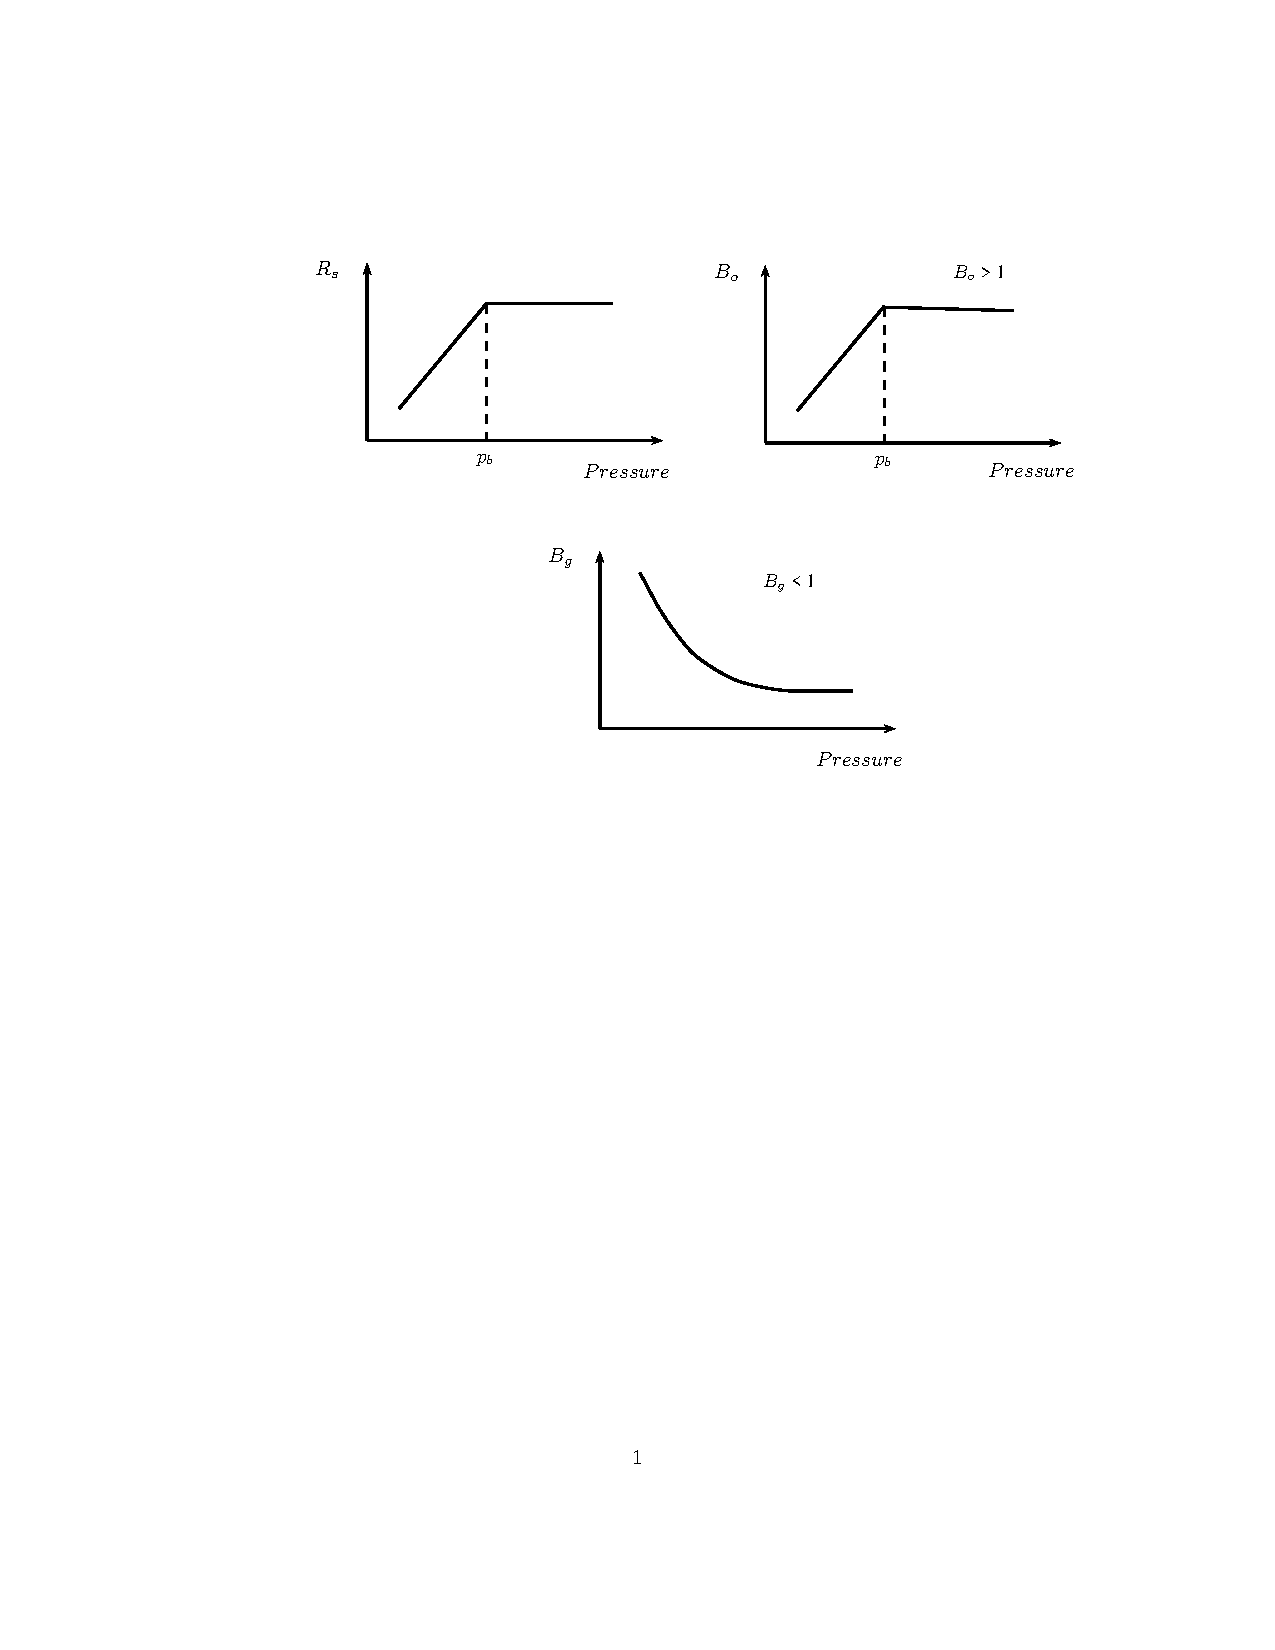
\includegraphics[scale=1]{Rs_Bo_Bg.pdf}
        \caption{$R_{s}$, $B_{o}$, $B_{g}$ behavior.}
        \label{Rs_Bo_Bg}
        \end{center}
    \end{figure}

    It is important to note that $B$ defined by Eq. \ref{Formation_Volume_Factor}\add[Murat \c{C}{\i}nar]{,} considering oil, \remove[Murat \c{C}{\i}nar]{this} is \change[Murat \c{C}{\i}nar]{correct}{valid} if \change[Murat \c{C}{\i}nar]{we have a}{oil is} single component or \remove[Murat \c{C}{\i}nar]{if we are talking about} "black-oil" with no dissolved gas ($R_{s}=0$). \change[Murat \c{C}{\i}nar]{However}{On the other hand}, Eq. \ref{Continuity_B_ct_Darcy} is \change[Murat \c{C}{\i}nar]{correct}{valid} for black-oil problems with $R_{s}\neq0$ provided that \change[Murat \c{C}{\i}nar]{we are}{the pressure is} above bubble-point. \remove[Murat \c{C}{\i}nar]{If we are above bubble-point,}Eq. \ref{Continuity_oil_Darcy} and Eq. \ref{Continuity_gas_Darcy} \change[Murat \c{C}{\i}nar]{will be}{becomes} identical\add[Murat \c{C}{\i}nar]{ if the pressure is above bubble point}.

    \change[Murat \c{C}{\i}nar]{Sometimes we write the flow equation}{In some cases, the flow equation is written} in terms of pseudo potential.

    \begin{equation}
        \psi =\int_{{{p}_{0}}}^{p}{\frac{1}{\gamma }dp}-\left( z'-{{z}_{0}}' \right)
    \label{Pseudo_Potential}
    \end{equation}

    where $z'$ is measured positive in the direction of gravity and ${{z}_{0}}'$ is the datum where \remove[Murat \c{C}{\i}nar]{we take as reference}${{p}_{0}}$ \add[Murat \c{C}{\i}nar]{is measured}. Also $\gamma=\mathbf{M}/\mathbf{L}^{2}\mathbf{T}^{2})$ and $\gamma=\gamma(p)$.

    \begin{equation*}
        \begin{split}
             \nabla \psi & =\nabla \int_{{{p}_{0}}}^{p}{\frac{1}{\gamma }dp}-\nabla \left( z'-{{z}_{0}}' \right) \\
            & =\frac{d}{dp}\left\{ \int_{{{p}_{0}}}^{p}{\frac{1}{\gamma }dp} \right\}\nabla p-\nabla z' \\
            & =\frac{1}{\gamma }\nabla p-\nabla z' \\
        \end{split}
    \end{equation*}

    Then,

    \begin{equation}
        \gamma \,\nabla \psi =\nabla p-\gamma \,\nabla z'
    \label{Pseudo_Potential_1}
    \end{equation}

    and

    \begin{equation}
        \frac{\partial \psi }{\partial t}=\frac{1}{\gamma }\frac{\partial p}{\partial t}
    \label{Pseudo_Potential_2}
    \end{equation}

    Using Eqs. \ref{Pseudo_Potential_1} and \ref{Pseudo_Potential_2} in Eq. \ref{Continuity_B_ct_Darcy} we obtain,

    \begin{equation}
        \nabla \cdot \left( \frac{\mathbf{k}\gamma }{B\mu }\nabla \psi  \right)=\frac{\phi {{c}_{t}}\gamma }{B}\frac{\partial \psi }{\partial t}
    \label{Pseudo_Potential_Final}
    \end{equation}

    If we consider that we have stress dependent reservoir, that is permeability decreases as the fluid pressure in the pores decreases, then
    \begin{equation*}
        \mathbf{k}=k\left( p \right)\widetilde{\mathbf{k}}
    \end{equation*}
        where the entries of $\widetilde{\mathbf{k}}$ are independent of pressure. It has been observed that tight (and geothermal) reservoirs are \remove[Murat \c{C}{\i}nar]{good} examples of stress dependent reservoirs. Then Eq. \ref{Pseudo_Potential_Final} \change[Murat \c{C}{\i}nar]{can be}{is} expressed as

    \begin{equation}
        \nabla \cdot \left( \frac{k\left( p \right)\widetilde{\mathbf{k}}\gamma }{B\mu }\nabla \psi  \right)=\frac{\phi {{c}_{t}}\gamma }{B}\frac{\partial \psi }{\partial t}
    \label{Pseudo_Potential_Final_Stress_dependent}
    \end{equation}
    \remove[Murat \c{C}{\i}nar]{
    It is important to note that Eq. 2.38 is non-linear because $\phi$, $c_{t}$, $\gamma$, $\mu$, $B$, and $k$ are all pressure dependent (or potential). To partially linearize the Eq. 2.38 (or Eq. 2.14), we normally define a pseudo pressure function if gravity effects are not important.}
    \Trcknote[Murat \c{C}{\i}nar]{Following paragraph is added.}A pseudo pressure function is defined to partially linearize Eq. \ref{Pseudo_Potential_Final_Stress_dependent} (or Eq. \ref{Continuity_B_ct_Darcy}) under the assumption that the gravity effects are not important.

    \begin{equation}
        m\left( p \right)=\int_{{{p}_{0}}}^{p}{\frac{k\left( p \right)}{\mu \left( p \right)B\left( p \right)}dp}
    \label{Pseudo_Pressure}
    \end{equation}

    \begin{equation}
        \nabla m\left( p \right)=\frac{d}{dp}m\left( p \right)\nabla p=\frac{k\left( p \right)}{\mu \left( p \right)B\left( p \right)}\nabla p
    \label{Pseudo_Pressure_1}
    \end{equation}

    \begin{equation}
        \frac{\partial m\left( p \right)}{\partial t}=\frac{k\left( p \right)}{\mu \left( p \right)B\left( p \right)}\frac{\partial p}{\partial t}
    \label{Pseudo_Pressure_2}
    \end{equation}

    If \change[Murat \c{C}{\i}nar]{we don't have gravity effects note that}{gravity effects are ignored,} Eq. \ref{Continuity_B_ct_Darcy} reduces to

    \begin{equation}
        \nabla \cdot \left( \frac{k\left( p \right)\widetilde{\mathbf{k}}}{B\left( p \right)\mu \left( p \right)}\nabla p \right)=\frac{\phi {{c}_{t}}}{B}\frac{\partial p}{\partial t}
    \label{Continuity_B_ct_Darcy_Nogravity}
    \end{equation}

    Using Eqs. \ref{Pseudo_Pressure}, \ref{Pseudo_Pressure_1}, and \ref{Pseudo_Pressure_2} in \ref{Continuity_B_ct_Darcy_Nogravity} gives

    \begin{equation}
        \nabla \cdot \left( \widetilde{\mathbf{k}}\nabla m\left( p \right) \right)=\frac{\phi \left( p \right){{c}_{t}}\left( p \right)\mu \left( p \right)}{k\left( p \right)}\frac{\partial m\left( p \right)}{\partial t}
    \label{Pseudo_Pressure_Continuity}
    \end{equation}

    Note Eq. \ref{Pseudo_Pressure_Continuity} is still non-linear. \remove[Murat \c{C}{\i}nar]{In} Eq. \ref{Pseudo_Potential_Final_Stress_dependent} \change[Murat \c{C}{\i}nar]{we have written our basic flow equations}{is the expression of basic flow equations} in terms of the potential $\psi$. Therefore, to partially linearize Eq. \ref{Pseudo_Potential_Final_Stress_dependent}, \change[Murat \c{C}{\i}nar]{we can define a "pseudo pressure" by}{a "pseudo pressure" is defined as}

    \begin{equation}
        m\left( \psi  \right)=\int_{{{\psi }_{0}}}^{\psi }{\frac{k\left( \psi  \right)\gamma \left( \psi  \right)}{\mu \left( \psi  \right)B\left( \psi  \right)}d\psi }
    \label{Pseudo_Pressure_potential}
    \end{equation}

    \subsection{Diffusivity equation for single phase gas flow - real gas flow}
    For \change[Murat \c{C}{\i}nar]{gas}{gases} $\mu$, $\rho$ are strong functions of pressure. Permeability typically is independent of pressure\change[Murat \c{C}{\i}nar]{ although}{, however,} at low pressures Klinkenberg effect may cause some pressure dependence in permeability and/or \change[Murat \c{C}{\i}nar]{if we have tight reservoirs}{tight reservoirs are considered} as discussed earlier. To account for the dependence of $k/ \mu B_{g}$ on pressure,\remove[Murat \c{C}{\i}nar]{we can use} Eq.\ref{Pseudo_Pressure} or \ref{Pseudo_Pressure_potential} \add[Murat \c{C}{\i}nar]{is used}. Note that Eq. \ref{Pseudo_Pressure_Continuity} is also valid for \change[Murat \c{C}{\i}nar]{real flow of}{flow of real} gases in porous media.\\

    With some modifications, the above procedure is the current approach used to derive the p.d.e. for gas flow. The method was first introduced in the literature by Al-Hussainy, Ramey and Crawford \cite{Al-Hussainy_1966_1}. Below \remove[Murat \c{C}{\i}nar]{we will derive}the p.d.e. \add[Murat \c{C}{\i}nar]{is derived} using Al-Hussainy et. al. \cite{Al-Hussainy_1966_1} approach. \remove[Murat \c{C}{\i}nar]{Since Eq. 2.32 is also valid for real gases, we have}\Trcknote[Murat \c{C}{\i}nar]{The following sentence is added.} Note that Eq. \ref{Continuity_B_ct_Darcy_Nogravity} holds for real gases. \change[Murat \c{C}{\i}nar]{Further, assuming}{Assuming} $k(p)\mathbf{k}$ is independent of pressure and same in all directions, then Eq. \ref{Continuity_B_ct_Darcy_Nogravity} \change[Murat \c{C}{\i}nar]{can be written as}{becomes}
    \begin{equation}
        \nabla \cdot \left( \frac{1}{B\left( p \right)\mu \left( p \right)}\nabla p \right)=\frac{\phi {{c}_{t}}}{kB}\frac{\partial p}{\partial t}
        \label{Gas_Flow_1}
    \end{equation}

    Since $B=\frac{{{\left( {{\rho }_{g}} \right)}_{SC}}}{{{\rho }_{g}}}$ and ${{\left( {{\rho }_{g}} \right)}_{SC}}$ is constant Eq. \ref{Gas_Flow_1} is equivalent to

    \begin{equation}
        \nabla \cdot \left( \frac{\rho }{\mu }\nabla p \right)=\frac{\phi {{c}_{t}}\rho }{k}\frac{\partial p}{\partial t}
        \label{Gas_Flow_2}
    \end{equation}

    Recall that $\rho$ for real gases is given by the following equation of state (EOS),

    \begin{equation}
        \rho =\frac{pM}{zRT}
        \label{Real_Gas_Law}
    \end{equation}

    Using Eq. \ref{Real_Gas_Law} in \ref{Gas_Flow_2} gives

    \begin{equation}
        \nabla \cdot \left( \frac{pM}{zRT\mu }\nabla p \right)=\frac{pM}{zRT}\frac{\phi {{c}_{t}}}{k}\frac{\partial p}{\partial t}
        \label{Gas_Flow_3}
    \end{equation}

    Since $M/RT$ is constant, then Eq. \ref{Gas_Flow_3} reduces to

    \begin{equation}
        \nabla \cdot \left( \frac{p}{z\mu }\nabla p \right)=\frac{\phi {{c}_{t}}p}{zk}\frac{\partial p}{\partial t}
        \label{Gas_Flow_4}
    \end{equation}

    Al-Hussainy et. al. \cite{Al-Hussainy_1966_1} defined the integral transform $m'(p)$ to be

    \begin{equation}
        m'\left( p \right)=2\int_{{{p}_{0}}}^{p}{\frac{p'}{\mu z}dp'}
        \label{Pseudo_Pressure_alhussainy}
    \end{equation}

    \begin{equation}
        \nabla m'\left( p \right)=\frac{2p}{\mu z}\nabla p
        \label{Pseudo_Pressure_alhussainy_1}
    \end{equation}

    \begin{equation}
        \frac{\partial m'}{\partial t}=2\frac{p}{\mu z}\frac{\partial p}{\partial t}
        \label{Pseudo_Pressure_alhussainy_2}
    \end{equation}

    Using Eqs. \ref{Pseudo_Pressure_alhussainy}, \ref{Pseudo_Pressure_alhussainy_1}, and \ref{Pseudo_Pressure_alhussainy_2} in \ref{Gas_Flow_4} gives,

    \begin{equation}
        \nabla \cdot \left[ \nabla m'\left( p \right) \right]=\frac{\phi {{c}_{t}}\mu \left( p \right)}{k}\frac{\partial m'\left( p \right)}{\partial t}
        \label{Gas_Flow_Final}
    \end{equation}

    \subsection{1-D Radial flow equation}
    Consider a completely penetrating well in an infinite porous medium of uniform thickness filled with a single phase fluid. Further assume that \change[Murat \c{C}{\i}nar]{we have axisymmetric flow}{flow is axisymmetric}, i.e., no variation in $\theta$-direction or in a plane $z'$=constant equipotential curves are circles - see Figure \ref{Radial_Flow},
    \begin{figure}
        \begin{center}
        \includegraphics[scale=1]{Radial_Flow.pdf}
        \label{Radial_Flow}
        \caption{Radial flow geometry.}
        \end{center}
    \end{figure}
    
    If reservoir is not horizontal, \remove[Murat \c{C}{\i}nar]{our general equation;} Eq. \ref{Continuity_B_ct_Darcy}, applies with $v_{\theta}=0$ and so Eq. \ref{Continuity_B_ct_Darcy} becomes in $r-z$ coordinates.
    
    \begin{equation}
        \begin{split}
    & \frac{1}{r}\frac{\partial }{\partial r}\left[ \frac{r{{k}_{r}}}{\mu B}\left( \frac{\partial p}{\partial r}-\gamma \frac{\partial z'}{\partial r} \right) \right] \\
    & +\frac{\partial }{\partial z}\left[ \frac{{{k}_{z}}}{\mu B}\left( \frac{\partial p}{\partial z}-\gamma \frac{\partial z'}{\partial z} \right) \right]=\frac{\phi {{c}_{t}}}{B}\frac{\partial p}{\partial t} \\
    \end{split}
        \label{Radial_Flow}
    \end{equation}
    
    \change[Murat \c{C}{\i}nar]{If we assume}{Now assume} $z=z'$ and $\theta=0$, then $\frac{\partial z'}{\partial r}=0$ 
    \begin{figure}
        \begin{center}
        \includegraphics[scale=1]{r_z.pdf}
        \end{center}
        \label{r_z}
        \caption{r-z coordinates.}
    \end{figure}    
  
    For a completely penetrating well, it is physically reasonable to assume $v_{z}\approx0$ ($k_{z}\ll k_{r}$), i.e.,
    \begin{equation}
    \begin{split}
    & {{v}_{z}}=-\frac{{{k}_{z}}}{\mu }\left( \frac{\partial p}{\partial z}-\gamma \frac{\partial z'}{\partial z} \right)=0\quad ;\quad \frac{\partial z'}{\partial z}=1 \\
    & \frac{\partial p}{\partial z}-\gamma =0\quad ;\quad p\left( {{z}_{2}} \right)=p\left( {{z}_{1}} \right)+\gamma \left( {{z}_{2}}-{{z}_{1}} \right)\quad {{z}_{z}}>{{z}_{1}} \\
    \end{split}
    \end{equation}    
 
        Then \remove[Murat \c{C}{\i}nar]{we arrive at}the general radial flow problem \add[Murat \c{C}{\i}nar]{becomes},
    \begin{equation}
        \frac{1}{r}\frac{\partial }{\partial r}\left( r\frac{{{k}_{r}}}{\mu B}\frac{\partial p}{\partial r} \right)=\frac{\phi {{c}_{t}}}{B}\frac{\partial p}{\partial t}
        \label{Radial_flow_general}
    \end{equation} 
    
    where $\phi$, $c_{t}$, $B$, $k_{r}$, and $\mu$ \change[Murat \c{C}{\i}nar]{can be}{are} functions of pressure.
    
    \change[Murat \c{C}{\i}nar]{Recalling our}{Recall} pseudo-pressure function defined as,
    
    \begin{equation}
        m\left( p \right)=\int_{{{p}_{b}}}^{p}{\frac{{{k}_{r}}\left( p \right)}{\mu \left( p \right)B\left( p \right)}dp}
        \label{Pseudo_pressure_r}
    \end{equation}     
    
    Using Eq. \ref{Pseudo_pressure_r}, \remove[Murat \c{C}{\i}nar]{we write} Eq. \ref{Radial_flow_general} \add[Murat \c{C}{\i}nar]{is written} as,
    
    \begin{equation}
        \frac{1}{r}\frac{\partial }{\partial r}\left( r\frac{\partial m\left( p \right)}{\partial r} \right)=\frac{\phi {{c}_{t}}\mu }{{{k}_{r}}}\frac{\partial m\left( p \right)}{\partial t}
        \label{Radial_flow_Pseudo_pressure}
    \end{equation}     
    
    \subsubsection{Dimensionless Variables} 
    In well testing \change[Murat \c{C}{\i}nar]{for two reasons, we are using dimensionless variables to prevent our results,}{dimensionless variables are used for two main reasons;}
    \begin{enumerate}[(i)]
        \item minimize number of variables \change[Murat \c{C}{\i}nar]{(find group parameters)}{(by grouping parameters)}
        \item provide general solutions
    \end{enumerate}    
    \change[Murat \c{C}{\i}nar]{If we define a dimensionless time}{Dimensionless time is defined as,}
    
    \begin{equation}
        {{t}_{D}}=\frac{{{k}_{i}}t}{{{\left( \phi {{c}_{t}}\mu  \right)}_{i}}r_{w}^{2}}
        \label{Dimensionless_time}
    \end{equation}        
    where subscript "$i$" refers to initial conditions, i.e.,
    \begin{equation*}
        k_{i} = k(p_{i})\,\,\,;\,\,\ \mu_{i}=\mu(p_{i})\,\,\,etc.
    \end{equation*}     
    
    here $p_{i}$ is the initial reservoir pressure (at some datum) and we assume $p_{i}$ is independent of $r$, then
    
    \begin{equation}
        \frac{\partial m}{\partial t}=\frac{\partial m}{\partial {{t}_{D}}}\frac{\partial {{t}_{D}}}{\partial t}=\frac{\partial m}{\partial {{t}_{D}}}\left( \frac{{{k}_{i}}}{{{\left( \phi {{c}_{t}}\mu  \right)}_{i}}r_{w}^{2}} \right)
        \label{Dimensionless_radial_1}
    \end{equation}     
    
    Using Eq. \ref{Dimensionless_radial_1} in Eq. \ref{Radial_flow_Pseudo_pressure}, and simplifying gives,\Trcknote[Murat \c{C}{\i}nar]{Typo corrected in the following equation}
    
    \begin{equation}
        r_{w}^{2}\left[ \frac{1}{r}\frac{\partial }{\partial r}\left( r\frac{\partial m\left( p \right)}{\partial r} \right) \right]=\left( \frac{\phi {{c}_{t}}\mu }{k} \right)\left[ \frac{{{k}_{i}}}{{{\left( \phi {{c}_{t}}\mu  \right)}_{i}}} \right]\frac{\partial m}{\partial {{t}_{D}}}
        \label{Dimensionless_radial_2}
    \end{equation}      
    
    \change[Murat \c{C}{\i}nar]{If we}{Now} define,
    \begin{equation}    
        {{r}_{D}}=\frac{r}{{{r}_{w}}}
        \label{Dimensionless_lenght}
    \end{equation}    
    
    and \add[Murat \c{C}{\i}nar]{dimensionless diffusivity,}
    
    \begin{equation}
        {{\eta }_{D}}=\frac{{k}/{\left( \phi {{c}_{t}}\mu  \right)}\;}{{{{k}_{i}}}/{{{\left( \phi {{c}_{t}}\mu  \right)}_{i}}}\;}
        \label{Dimensionless_diffusivity}
    \end{equation}        
    
    then\remove[Murat \c{C}{\i}nar]{we can write} Eq. \ref{Dimensionless_radial_2} \change[Murat \c{C}{\i}nar]{as}{becomes}
    
    \begin{equation}
        \frac{1}{{{r}_{D}}}\frac{\partial }{\partial {{r}_{D}}}\left( {{r}_{D}}\frac{\partial m\left( p \right)}{\partial {{r}_{D}}} \right)=\frac{1}{{{\eta }_{D}}}\frac{\partial m\left( p \right)}{\partial {{t}_{D}}}
        \label{Dimensionless_radial_3}
    \end{equation}       
    
    If $\frac{1}{{{\eta }_{D}}}=0$, then Eq. \ref{Dimensionless_radial_3} is a linear p.d.e. .
    
    \subsubsection{Slightly compressible fluid of constant compressibility}
    
    \change[Murat \c{C}{\i}nar]{If we assume}{Consider} production at a specified rate q; i.e.,
    \begin{figure}
        \begin{center}
        \includegraphics[scale=1]{Production_Full.pdf}
        \label{Production_Full}
        \caption{Production from a vertical full penetrating well. Volumetric flux, q, into the wellbore (flow out of the reservoir the boundary represented by wellbore).}
        \end{center}
    \end{figure}    
    
    Flow rate out = $qB=\int\limits_{S}{\mathbf{v}\,\mathbf{n}\,dS}$ and $\mathbf{n}$ is the unit outward normal to $S$ and is equal to 
    
    \begin{equation*}
        \begin{split}
        & \mathbf{n}=-{{i}_{r}}+0{{i}_{\theta }}+0{{i}_{z}}=\left( 1,0,0 \right) \\
        & \mathbf{v}=\left( {{v}_{r}}+{{v}_{\theta }}+{{v}_{z}} \right) \\
        \end{split}
    \end{equation*}
    
    \begin{equation*}
        \begin{split}
             qB&=\int\limits_{S}{-{{\left. {{v}_{r}} \right|}_{r={{r}_{w}}}}}dS\quad ;\quad ds={{r}_{w}}d\theta dz \\
             qB&=\int_{0}^{2\pi }{\int_{0}^{h}{{{\left( -{{v}_{r}} \right)}_{{{r}_{w}}}}{{r}_{w}}}}d\theta dz \\
             q&={{\int_{0}^{2\pi }{\int_{0}^{h}{\frac{k}{\mu B}\left( r\frac{\partial p}{\partial r} \right)}}}_{r={{r}_{w}}}}d\theta dz \\
             q&=2\pi {{\int_{0}^{h}{\left( r\frac{\partial m}{\partial r} \right)}}_{{{r}_{w}}}}dz \\
        \end{split}
    \end{equation*}    
    
    \change[Murat \c{C}{\i}nar]{If}{Now} we assume \add[Murat \c{C}{\i}nar]{that} variation of $r\frac{\partial m\left( p \right)}{\partial r}$ in z-direction is insignificant or
    \begin{equation*}
    {{\int\limits_{0}^{h}{\left( r\frac{\partial m\left( p \right)}{\partial r} \right)}}_{{{r}_{w}}}}dz={{\left( r\frac{\partial m\left( p \right)}{\partial r} \right)}_{{{r}_{w}},\widehat{z}}}h
    \end{equation*}  
    where $\widehat{z}$ is a mean value between $0\leq \widehat{z} \leq h$. Then the boundary condition is
    
    
    \begin{equation}
        q=2\pi h{{\left( r\frac{\partial m\left( p \right)}{\partial r} \right)}_{{{r}_{w}}}}
        \label{Well_boundary}
    \end{equation}      
    
    \change[Murat \c{C}{\i}nar]{If we define}{Define,}
    \begin{equation}    
        \begin{split}
         {{m}_{D}}&=\frac{2\pi h\left[ m\left( {{p}_{i}} \right)-m\left( p \right) \right]}{q} \\
        & =\frac{h}{q}\left[ m\left( {{p}_{i}} \right)-m\left( p \right) \right] \\
        & =\frac{h}{q}\int\limits_{p}^{{{p}_{i}}}{\frac{k\left( p \right)}{\mu \left( p \right)B\left( p \right)}dp} \\
        \end{split}
        \label{mD_definition}
    \end{equation}      
       
    Then \change[Murat \c{C}{\i}nar]{one}{we} can show that Eqs. \ref{Dimensionless_radial_3} and \ref{Well_boundary}\change[Murat \c{C}{\i}nar]{, respectively, can be}{ is} written as
    \begin{equation}
            \frac{1}{{{r}_{D}}}\frac{\partial }{\partial {{r}_{D}}}\left( {{r}_{D}}\frac{\partial {{m}_{D}}}{\partial {{r}_{D}}} \right)=\frac{1}{{{\eta }_{D}}}\frac{\partial {{m}_{D}}}{\partial {{t}_{D}}}
        \label{Dimensionless_radial_4}
    \end{equation}        
    \begin{equation}
            {{\left( {{r}_{D}}\frac{\partial {{m}_{D}}}{\partial {{r}_{D}}} \right)}_{{{r}_{D}}=1}}=-1
        \label{Well_boundary_2}
    \end{equation}        
    Note that $r_{D}=1$ corresponds to $r=r_{w}$.
    Initial condition, $p=p_{i}$ at values of $r$ at $\widehat{z}$. 
    $m_{D}=0$ at $t_{D}=0$ then,
    \begin{equation}
        {{\left. p\left( r,t \right) \right|}_{t=0}}={{p}_{i}}    
        \label{initial_condition}
    \end{equation}       
    
    \change[Murat \c{C}{\i}nar]{Since we consider an infinite reservoir, then}{Infinite acting reservoir is considered implying,}
    \begin{equation*}
        \underset{r\to \omega }{\mathop{\lim }}\,p\left( r,t \right)={{p}_{i}}
    \end{equation*}
    
    which corresponds to
    \begin{equation}
        \underset{{{r}_{D}}\to \infty }{\mathop{\lim }}\,{{m}_{D}}\left( {{r}_{D}},{{t}_{D}} \right)=0
        \label{initial_condition_md}
    \end{equation}    
    
    In summary, \change[Murat \c{C}{\i}nar]{we have the following IBVP,}{the following initial boundary value problem (IBVP) is achieved with the appropriate boundary conditions.}
    \begin{equation}
        \frac{1}{{{r}_{D}}}\frac{\partial }{\partial {{r}_{D}}}\left( {{r}_{D}}\frac{\partial {{m}_{D}}}{\partial {{r}_{D}}} \right)=\frac{1}{{{\eta }_{D}}}\frac{\partial {{m}_{D}}}{\partial {{t}_{D}}}
        \label{Dimensionless_radial_md_Sum}
    \end{equation}      
    
    \begin{equation}
        {{\left( {{r}_{D}}\frac{\partial {{m}_{D}}}{\partial {{r}_{D}}} \right)}_{{{r}_{D}}=1}}=-1
        \label{Boundary_1_sum}
    \end{equation}     
    
    \begin{equation}
        \underset{{{r}_{D}}\to \infty }{\mathop{\lim }}\,{{m}_{D}}\left( {{r}_{D}},{{t}_{D}} \right)=0
        \label{Boundary_2_sum}
    \end{equation}    
    
    \begin{equation}
        {{m}_{D}}\left( {{r}_{D}},{{t}_{D}}=0 \right)=0
        \label{Initial_con_sum}
    \end{equation}       
    
    Eqs. \ref{Dimensionless_radial_md_Sum}-\ref{Initial_con_sum} lead to give a complete mathematical description of \change[Murat \c{C}{\i}nar]{our}{the} physical problem. Because of ${{\eta }_{D}}$ term, it is a non-linear IBVP. It can also be solved analytically (see Kale and Mattar\cite{Kale_1980_1} or Peres et.al.\cite{Peres_1990_1})
    
    \change[Murat \c{C}{\i}nar]{Let's now, for}{For} simplicity, assume that variations in $k$, $\phi$, $c_{t}$, and $B$ are small ("negligible") for the pressure change considered. \change[Murat \c{C}{\i}nar]{wit this assumption}{Then,}
     \begin{equation}
        {{\eta }_{D}}=\frac{\left( {k}/{\phi {{c}_{t}}\mu }\; \right)}{{{\left( {k}/{\phi {{c}_{t}}\mu }\; \right)}_{{{p}_{i}}}}}\approx 1
        \label{assumption}
    \end{equation}     
    
    and
    
    \begin{equation}
        {{\eta }_{D}}=\frac{\left( {k}/{\phi {{c}_{t}}\mu }\; \right)}{{{\left( {k}/{\phi {{c}_{t}}\mu }\; \right)}_{{{p}_{i}}}}}\approx 1
        \label{assumption}
    \end{equation}        
    
    \begin{equation}
        m\left( {{p}_{i}} \right)-m\left( p \right)=\int_{p}^{{{p}_{i}}}{\frac{k\left( p \right)}{\mu \left( p \right)B\left( p \right)}dp\approx \frac{{{k}_{i}}}{{{\mu }_{i}}{{B}_{i}}}}\left( {{p}_{i}}-p \right)
        \label{assumption_2}
    \end{equation}     
    
    and then it follows from Eq. \ref{mD_definition} that
    
    \begin{equation}
        {{m}_{D}}=\frac{{{k}_{i}}h\left( {{p}_{i}}-p \right)}{q{{B}_{i}}{{\mu }_{i}}}={{p}_{D}}=\frac{kh\left( {{p}_{i}}-p \right)}{qB\mu }
        \label{mD_to_pD}
    \end{equation}     
    
    \change[Murat \c{C}{\i}nar]{which is the normal}{that is the} definition of dimensionless pressure $p_{D}$ in well testing.
    Considering $\frac{1}{{{\eta }_{D}}}\approx 1$ in Eq. \ref{Dimensionless_radial_md_Sum}, we have
    
    \begin{equation}
        \frac{1}{{{r}_{D}}}\frac{\partial }{\partial {{r}_{D}}}\left( {{r}_{D}}\frac{\partial {{m}_{D}}}{\partial {{r}_{D}}} \right)=\frac{\partial {{m}_{D}}}{\partial {{t}_{D}}}
        \label{Dimensionless_radial_md_Sum_lin}
    \end{equation}

    \begin{equation}
        {{\left( {{r}_{D}}\frac{\partial {{m}_{D}}}{\partial {{r}_{D}}} \right)}_{{{r}_{D}}=1}}=-1
        \label{Boundary_1_sum_lin}
    \end{equation}

    \begin{equation}
        \underset{{{r}_{D}}\to \infty }{\mathop{\lim }}\,{{m}_{D}}\left( {{r}_{D}},{{t}_{D}} \right)=0
        \label{Boundary_2_sum_lin}
    \end{equation}

    \begin{equation}
        {{m}_{D}}\left( {{r}_{D}},{{t}_{D}}=0 \right)=0
        \label{Initial_con_sum_lin}
    \end{equation}      
    
    Note that Eq. \ref{Dimensionless_radial_md_Sum_lin} is a linear p.d.e. . We seek a solution to the IBVP given by Eqs. \ref{Dimensionless_radial_md_Sum_lin} - \ref{Initial_con_sum_lin}. To find a solution we assume that
    \begin{equation*}    
    {{m}_{D}}={{m}_{D}}\left( {{\varepsilon }_{D}} \right)
    \end{equation*}    
    where
    \begin{equation*}
    {{\varepsilon }_{D}}=\frac{r_{D}^{2}}{4{{t}_{D}}}={{\varepsilon }_{D}}\left( {{r}_{D}},{{t}_{D}} \right)
    \end{equation*}     
    
    %\nomenclature[1]{$R$}{Ideal gas constant {$(8.314 J/gmol \cdot K)$}}%
    %\nomenclature{${\alpha }$}{Reaction order}%
    %\printnomenclature

    \bibliographystyle{plain}
    \bibliography{References}
%
\end{document}
